\documentclass[aspectratio=169,13pt,t] {beamer}
%
% Choose how your presentation looks.
%
% For more themes, color themes and font themes, see:
% http://deic.uab.es/~iblanes/beamer_gallery/index_by_theme.html
%
\mode<presentation>
{
  \usetheme{Madrid}      % or try Darmstadt, Madrid, Warsaw, ...
  \usecolortheme{beaver} % or try albatross, beaver, crane, ...
  \usefonttheme{serif}  % or try serif, structurebold, ...
%  \setbeamertemplate{navigation symbols}{}
  \setbeamertemplate{caption}[numbered]
  \setbeamertemplate{items}[default]
} 

\usepackage[,UTF8,linespread=1.2]{ctex}
\usepackage{wrapfig}
\usepackage{caption}
\captionsetup[figure]{name=图,labelsep=period}
\usepackage[,most]{tcolorbox}
\usepackage{picinpar}


\usepackage{xcolor}
\definecolor{xy_blue}{cmyk}{0.6,0.35,0.0,0.4}
\definecolor{xy_orange}{cmyk}{0.0,0.7,1.0,0.0}
\definecolor{xy_green}{cmyk}{0.2,0.0,1.0,0.15}
\xdefinecolor{xy_gold}{RGB}{135,103,79}
\xdefinecolor{xy2_gold}{cmyk}{0,0.35,0.75,0.05}


\setbeamercolor{section number projected}{fg=red,bg=red!20}%控制球的颜色
\setbeamercolor{subsection number projected}{fg=blue,bg=blue!40}
\setbeamercolor{item}{fg=xy_gold} %设置列表项颜色

\usepackage{amsthm}
\newtheorem{peroration}{结论：}
\newtheorem{exploration}{探究：}
\newtheorem{prooft}{证明：}
\newtheorem{question}{问题}
\newtheorem*{solve}{解:} 
\newtheorem{instance}{例}   % 解：独立计数器
\BeforeBeginEnvironment{peroration}{%
	\setbeamercolor{block title}{bg=xy_green,fg=white}
	\setbeamercolor{block body}{bg=xy_green!10}
}
\AfterEndEnvironment{peroration}{
	\setbeamercolor{block title}{bg=xy_blue,fg=white}
	\setbeamercolor{block body}{bg=xy_blue!10}
}
\BeforeBeginEnvironment{exploration}{%
	\setbeamercolor{block title}{bg=xy_orange,fg=white}
	\setbeamercolor{block body}{bg=xy_orange!10}
}
\AfterEndEnvironment{peroration}{
	\setbeamercolor{block title}{bg=xy_blue,fg=white}
	\setbeamercolor{block body}{bg=xy_blue!10}
}
\BeforeBeginEnvironment{solution}{%
	\setbeamercolor{block title}{bg=xy_green,fg=white}
	\setbeamercolor{block body}{bg=xy_green!10}
}
\AfterEndEnvironment{solution}{
	\setbeamercolor{block title}{bg=xy_green,fg=white}
	\setbeamercolor{block body}{bg=xy_green!10}
}
\BeforeBeginEnvironment{prooft}{%
	\setbeamercolor{block title}{bg=xy_green,fg=white}
	\setbeamercolor{block body}{bg=xy_green!10}
}
\AfterEndEnvironment{prooft}{
	\setbeamercolor{block title}{bg=xy_green,fg=white}
	\setbeamercolor{block body}{bg=xy_green!10}
}
\BeforeBeginEnvironment{question}{%
	\setbeamercolor{block title}{bg=xy_orange,fg=white}
	\setbeamercolor{block body}{bg=xy_orange!10}
}
\AfterEndEnvironment{question}{
	\setbeamercolor{block title}{bg=xy_green,fg=white}
	\setbeamercolor{block body}{bg=xy_green!10}
}
\BeforeBeginEnvironment{solve}{%解：
	\begingroup
	\setbeamercolor{block title}{bg=xy_orange!60,fg=white}
	\setbeamercolor{block body}{bg=xy_orange!10}
}
\AfterEndEnvironment{solve}{%解：
	\endgroup
}

\setbeamercolor{prooft}{fg=red, bg=green!10}       % 标题颜色
\setbeamercolor{prooft body}{fg=red, bg=red!5}  % 内容块背景
\setbeamerfont{prooft head}{series=\bfseries}       % 标题字体
\setbeamerfont{question body}{shape=\upshape}         % 内容字体
\renewcommand{\thefigure}{\arabic{figure}}

\newtcolorbox{summarybox}[1][]{
	colback=purple!10,
	colframe=purple!70!black,
	fonttitle=\bfseries,
	title=#1,
	arc=1mm,
	boxrule=0pt,drop shadow,
	left=2mm, right=2mm, top=2mm, bottom=2mm,
}
\newtcolorbox{summarybox-answer}{
	width=0.9\textwidth,
	colback=white,
	blanker,
	borderline west={2pt}{20pt}{cyan},
	left=10mm, right=2mm, top=2mm, bottom=2mm,
	}
\title[3.1.1函数的概念]{3.1.1函数的概念}
\author[好好学习，努力向上]{}
\institute{}
\date{2026.10.8}
%\setbeamertemplate{theorems}[numbered]
\theoremstyle{definition}
\newtheorem{exam}{例}
\AtBeginSection[]
{
  \begin{frame}<beamer>
    \frametitle{本节主要内容}
    \tableofcontents[currentsection,currentsubsection]
  \end{frame}
}

\AtBeginDocument{
	\setlength{\abovedisplayskip}{3pt}
	\setlength{\belowdisplayskip}{3pt}
	\setbeamertemplate{theorems}[numbered]
}

\begin{document}
\begin{frame}{}
	\titlepage
\end{frame}

\begin{frame}{内容概览}
	\tableofcontents
\end{frame}

\section{问题情景}
\begin{frame}{问题情景}
	\begin{question}
	\begin{wrapfigure}{r}{6cm}
		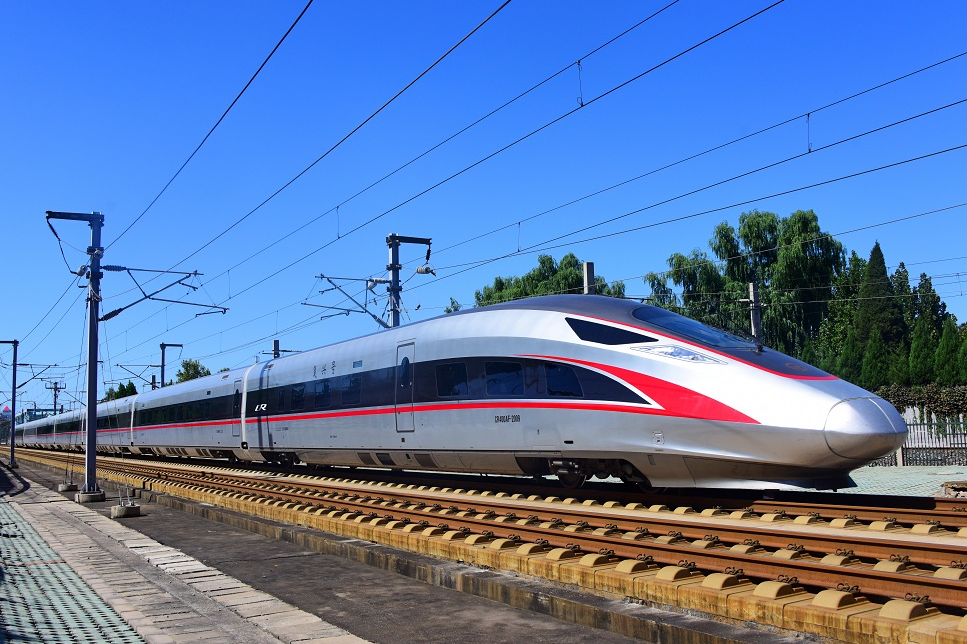
\includegraphics[scale=0.18]{Figures/fuxinghao.png}
	\end{wrapfigure}
	某“复兴号”高速列车加速到 \(350\text{ km/h}\) 后保持匀速运行半小时. 这段时间内，列车行进的路程 \(S\)（单位：\(\text{km}\)）与运行时间 \(t\)（单位：\(\text{h}\)）的关系可以表示为
	\[
	S = 350t.
	\]
	这里，\(t\) 和 \(S\) 是两个变量，而且对于 \(t\) 的每一个确定的值，\(S\) 都有唯一确定的值与之对应，所以 \(S\) 是 \(t\) 的函数.
	
	~
	
	~
\end{question}
\end{frame}


\begin{frame}{问题情景}
	\begin{question}
		某电气维修公司要求工人每周工作至少 1 天，至多 6 天. 如果公司确定的工资标准是每人每天 350 元，而且每周付一次工资，那么你认为该公司怎样确定一个工人每周的工资？一个工人的工资 \(w\)（单位：元）是他工作天数 \(d\) 的函数吗？
	\end{question}
	 
	
\end{frame}

\begin{frame}{问题情景}
	\vspace{-1.5em}
	\begin{question}
		\upshape 图 \ref{fig:fig01} 是某市某日的空气质量指数（Air Quality Index，简称 AQI）变化图. 如何根据该图确定这一天内任一时刻 \(t\text{ h}\) 的空气质量指数（AQI）的值 \(I\)？你认为这里的 \(I\) 是 \(t\) 的函数吗？
	\end{question}
	\begin{figure}
		\centering
		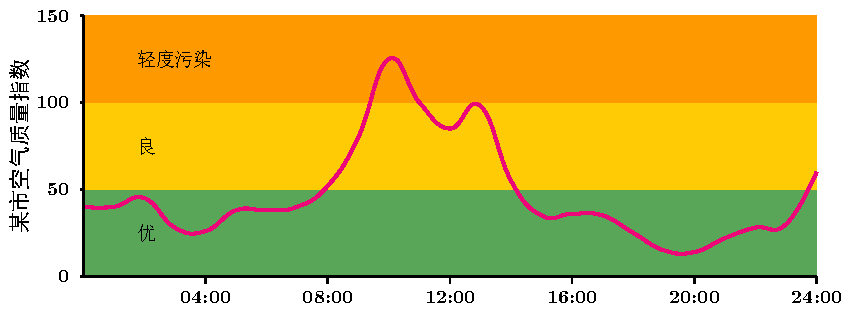
\includegraphics[scale=0.9,]{Figures/aqi_pgf.pdf}
		\caption{}
		\label{fig:fig01}
	\end{figure}
	

\end{frame}


\begin{frame}{问题情景}
	\begin{question}
		 国际上常用恩格尔系数 \(r\) {\upshape (\(r = \dfrac{\text{食物支出金额}}{\text{总支出金额}} \times 100\%\))}\rule[-15pt]{0pt}{2pt} 反映一个地区人民生活质量的高低，恩格尔系数越低，生活质量越高. 表 \ref{table:tab1} 是我国某省城镇居民恩格尔系数变化情况，从中可以看出，该省城镇居民的生活质量越来越高.
	\end{question}
	
	
	\begin{table}[h]
		\centering	
		\renewcommand{\arraystretch}{1.3}
		
		\begin{tabular}{|c|c|c|c|c|c|c|c|c|c|c|}
			\hline
			年份 \(y\) & 2012 & 2013 & 2014 & 2015 & 2016 & 2017 & 2018	& 2019 & 2020 & 2021 \\ \hline
			恩格尔系数 \(r\) (\%) & 32.0 & 30.1 & 30.0 & 29.7 & 29.3 & 28.6 & 27.7 & 27.6 & 29.2 & 28.6 \\ \hline
		\end{tabular}
		\caption {我国某省城镇居民恩格尔系数变化情况}
		\label{table:tab1}
	\end{table}
\end{frame}

\section{函数的概念}
\begin{frame}
	\begin{summarybox}[归纳]
		上述问题 1\(\sim\)问题 4 中的函数有哪些共同特征？由此你能概括出函数概念的本质特征吗？
	\end{summarybox}
	\pause
\begin{summarybox-answer}
	上述问题的共同特征有：
	\begin{enumerate}[(\arabic*)]
		\item 都包含两个非空数集，用 \(A, B\) 来表示；
		\item 都有一个对应关系；
		\item 尽管对应关系的表示方法不同，但它们都有如下特性：对于数集 \(A\) 中的任意一个数 \(x\)，按照对应关系，在数集 \(B\) 中都有唯一确定的数 \(y\) 和它对应.
	\end{enumerate}
\end{summarybox-answer}		

\end{frame}

\begin{frame}
	\begin{definition}[函数的定义]
		一般地，设 \(A, B\) 是非空的实数集，如果对于集合 \(A\) 中的任意一个数 \(x\)，按照某种确定的对应关系 \(f\)，在集合 \(B\) 中都有唯一确定的数 \(y\) 和它对应，那么就称 \(f: A \to B\) 为从集合 \(A\) 到集合 \(B\) 的一个\textbf{函数}（function），记作
		\[
		y = f(x), \quad x \in A.
		\]
		其中，\(x\) 叫做自变量，\(x\) 的取值范围 \(A\) 叫做函数的\textbf{定义域}（domain）；与 \(x\) 的值相对应的 \(y\) 值叫做函数值，函数值的集合 \(\{f(x) \mid x \in A\}\) 叫做函数的\textbf{值域}（range）.
	\end{definition}

		
		

\end{frame}

\begin{frame}
	\begin{example}
		 函数的解析式是舍弃问题的实际背景而抽象出来的，它所反映的两个量之间的对应关系，可以广泛地用于刻画一类事物中的变量关系和规律. 例如，正比例函数 \(y = kx (k \neq 0)\) 可以用来刻画匀速运动中路程与时间的关系、一定密度的物体的质量与体积的关系、圆的周长与半径的关系等.
		
		试构建一个问题情境，使其中的变量关系可以用解析式 \(y = x(10 - x)\) 来描述.
	\end{example}
\vspace{-2ex}
	\begin{solve}<2->
	把 \(y = x(10 - x)\) 看成二次函数，那么它的定义域是 \(\mathbf{R}\)，值域是 \(B = \{y \mid y \leqslant 25\}\). 对应关系 \(f\) 把 \(\mathbf{R}\) 中的任意一个数 \(x\)，对应到 \(B\) 中唯一确定的数 \(x(10 - x)\).
	
	如果对 \(x\) 的取值范围作出限制，例如 \(x \in \{x \mid 0 < x < 10\}\)，那么可以构建如下情境：
	
	长方形的周长为 20，设一边长为 \(x\)，面积为 \(y\)，那么 \(y = x(10 - x)\).
	
	其中，\(x\) 的取值范围是 \(A = \{x \mid 0 < x < 10\}\)，\(y\) 的取值范围是 \(B = \{y \mid 0 < y \leqslant 25\}\). 对应关系 \(f\) 把每一个长方形的边长 \(x\)，对应到唯一确定的面积 \(x(10 - x)\).
	\end{solve}
\end{frame}

\begin{frame}{布置作业}
	P63---64练习： 1---4
	
	
\end{frame}

\end{document}
